%\section{Distribution of IVOA Virtual Observatories Worlwide and its Projects}
\section{IVOA Virtual Observatories Worldwide}
\label{sec:ivoa}

Astronomy has always been a data-driven science, and therefore,
the digital revolution have completely change the astronomical practice.
In fact, the actual presence of the astronomer on site is every
day less required for performing observations, and data reduction process
is migrating out of the observatories, and international data sharing
and collaboration are becoming common practices in the community.

However, the paradigm change 
does not stop here, because astronomers have to front the main challenge of
21st century science: the data deluge. It is a fact that astronomical data will
strongly increase both in size and in quantity on the next decade due to various
reasons, including the building of large projects like ALMA and E-ELT, 
the improvement and deployment of new instruments, and the execution of 
large astronomical surveys like the LSST project.
The effort needed to process all this data will be enormous both
scientifically and in terms of computational capacity. 
For instance, simple search and access procedures could become highly expensive
when too many files are available in the database.

Consequently, is desirable to distribute the scientific and the computational 
load in several centers, each one specialized on certain data and instruments
to avoid redundancy of observations and work. However, this distributed work
should be organized to be able to interoperate between centers.
In this context, organizing the inherent diversity of several countries working together, 
with different goals, working-style and budgets is the central objective of
the IVOA.


%\subsection{Organizations}
%\begin{itemize}
%	\item \textbf{CVO}
%	\item Canadian Astronomy Data Centre
%	\item \textbf{VAO}
%	\item National Science Foundation, NSF
%	\item National Aeronautics and Space Administration, NASA 
%	\item Associated Universities, Inc, AUI.
%	\item Association of Universities for Reseach in Astronomy, AURA
%	\item \textbf{BRAVO}
%	\item Brazilian Astronomical Society, SBA
%	\item National Institue for Science and Technology in Astrophysics, INCT-A
%	\item \textbf{ChiVO}
%	\item 5 universities, supported by ALMA, REUNA
%	\item \textbf{NOVA}
%	\item 8 institutions, National Universitiy of La Plata, Faculty of Astronomical 
%		Sciences and Geophysics of la Plata
%	\item \textbf{ArVO}
%	\item Digital First Byurakan Survey, DFBS
%	\item \textbf{AstroGrid}
%	\item Particle Physics and Astronomy and Research Council  (PPARC)
%	\item Sciency \& Technology Facilities Council (STFC)
%	\item \textbf{ESA-VO}
%	\item Study
%	\item \textbf{EURO-VO}
%	\item Continuation of Astrophysical Virtual Observatory, European Commision and six organization
%	\item \textbf{GAVO}
%	\item Federal Ministry of Education and Research (BMBF)
%	\item \textbf{SVO}
%	\item Centro de Astrobiología (INTA-CSIC)
%	\item Artificial Intelligence Department of the National University of Distance Education
%	\item University of Cádiz and Center of Scientific and Academic Services of Catalonia (CESCA)
%	\item \textbf{VObs.it}
%	\item Italian National Institute for Astrophysics
%	\item Information System Units
%	\item \textbf{Ukrainian}
%	\item Ukrainian Astronomical Association (UAA)
%	\item \textbf{SA$^3$}
%	\item National Research Fundation
%	\item South African Astronomical Observatory
%	\item Hartebeesthoek Radio Astronomy Observatory
%	\item Square Kilometer Array South Africa 
%	\item \textbf{China-VO}
%	\item National Astronomical Observatories
%	\item Chinese Academy of Sciences
%	\item \textbf{JVO}
%	\item National Astronomical Observatory of Japan
%	\item Fujitsu
%	\item \textbf{VOI}
%	\item Inter University Center for Astronomy and Astrophysics
%	\item Ministry of Communication and Information Technology
%	\item \textbf{Aus-VO}
%	\item Linkage Infrastructure, Equipment and Facilities
%\end{itemize}

\scriptsize
\begin{table}[h]
\centering
%\begin{tabular}{|p{7cm}|p{7cm}|}
\begin{tabular}{|l|l|l|}
	\hline
	\textbf{Project} & \textbf{Since} & %\textbf{Organization} & % \textbf{Institutions Acronyms} & 
\textbf{URL} \\
	\hline
	Aus-VO (Australia) & 2002 & %Partnership of 10 Universities/Institutes  & 
		\url{http://aus-vo.org.au/} \\
	\hline
   CVO (Canada) & 2002 & %Governmental Initiative + 1 partner & % CADC, NRC, CSA &
   	\url{http://www.cadc-ccda.hia-iha.nrc-cnrc.gc.ca} \\
%	EURO-VO (Europe) & 
%& & \url{http://www.euro-vo.org/} \\
	\hline
	GAVO (German) & 2002 & % Partnership of 5 Universities/Institutes &   
		\url{http://www.g-vo.org/} \\
	\hline
	VO-France (France) & 2002 & % & 
		\url{http://www.france-vo.org/} \\
	\hline
	RVO (Russia) & 2002 & % &  
		\url{http://www.inasan.rssi.ru/eng/rvo/} \\
	\hline
	US-VAO (United States) & 2002 & %  &
		 \url{http://www.usvao.org/} \\
	\hline
	VOI (India) & 2002 & %  & 
		\url{http://vo.iucaa.ernet.in/~voi/} \\
	\hline
	AstroGrid (UK) & 2002 & %Consortium of 7 University/Institutes & %CU,EU,LU,UM,RAL,UCL,UB & 
		\url{http://www.astrogrid.org/} \\
	\hline
   China-VO (China) & 2003 & % Partnership of 4 Universities/Institutes  & 
   \url{http://www.china-vo.org/} \\
	\hline
	JVO (Japan) & 2003 &% &  
		\url{http://jvo.nao.ac.jp/}\\
	\hline
	VObs.it (Italy) & 2003 & % & 
		\url{http://vobs.astro.it/} \\
	\hline
	HVO (Hungary) & 2003 & %&
 		\url{http://hvo.elte.hu/en/} \\
	\hline
	SVO (Spain) & 2005 & % &  
		\url{http://svo.cab.inta-csic.es/} \\
	\hline
	ARVO (Armenia) & 2006 & %Observatory Initiative + 1 partner & % BAO, ANAS & 
		\url{http://www.aras.am/Arvo/arvo.htm} \\
	\hline
	BRAVO (Brazil) & 2009 & %Governmental Initiative + 4 partners &  %INCT-A,MCT,USP,UFSC,LNA & 
		\url{http://www.lna.br/bravo/} \\
	\hline
	UkrVO (Ukraine) & 2011 & % &  
		\url{http://www.ukr-vo.org/} \\
	\hline
	NOVA (Argentina) & 2011 & %Governmental Initiative + 9 partners  & % CONICET,CASLEO,IALP,IAFE,OAC,IAR,ICATE,UNPL,IATE & 
		\url{http://nova.conicet.gov.ar/} \\
	\hline
	SA$^3$ (South Africa) & 2013 & %  & 
		\url{http://www.sa3.ac.za/} \\
	\hline
    ChiVO (Chile) & 2013 & %Partnership of 7 Universities/Institutes & %UTFSM,UChile,PUC,UdeC,USACH,REUNA,ALMA & 
		\url{http://www.chivo.cl/} \\
	\hline
\end{tabular}
\caption{IVOA's partners.}
\label{table:partners}
\end{table}
\normalsize

\begin{figure}%[h]
\begin{center}
	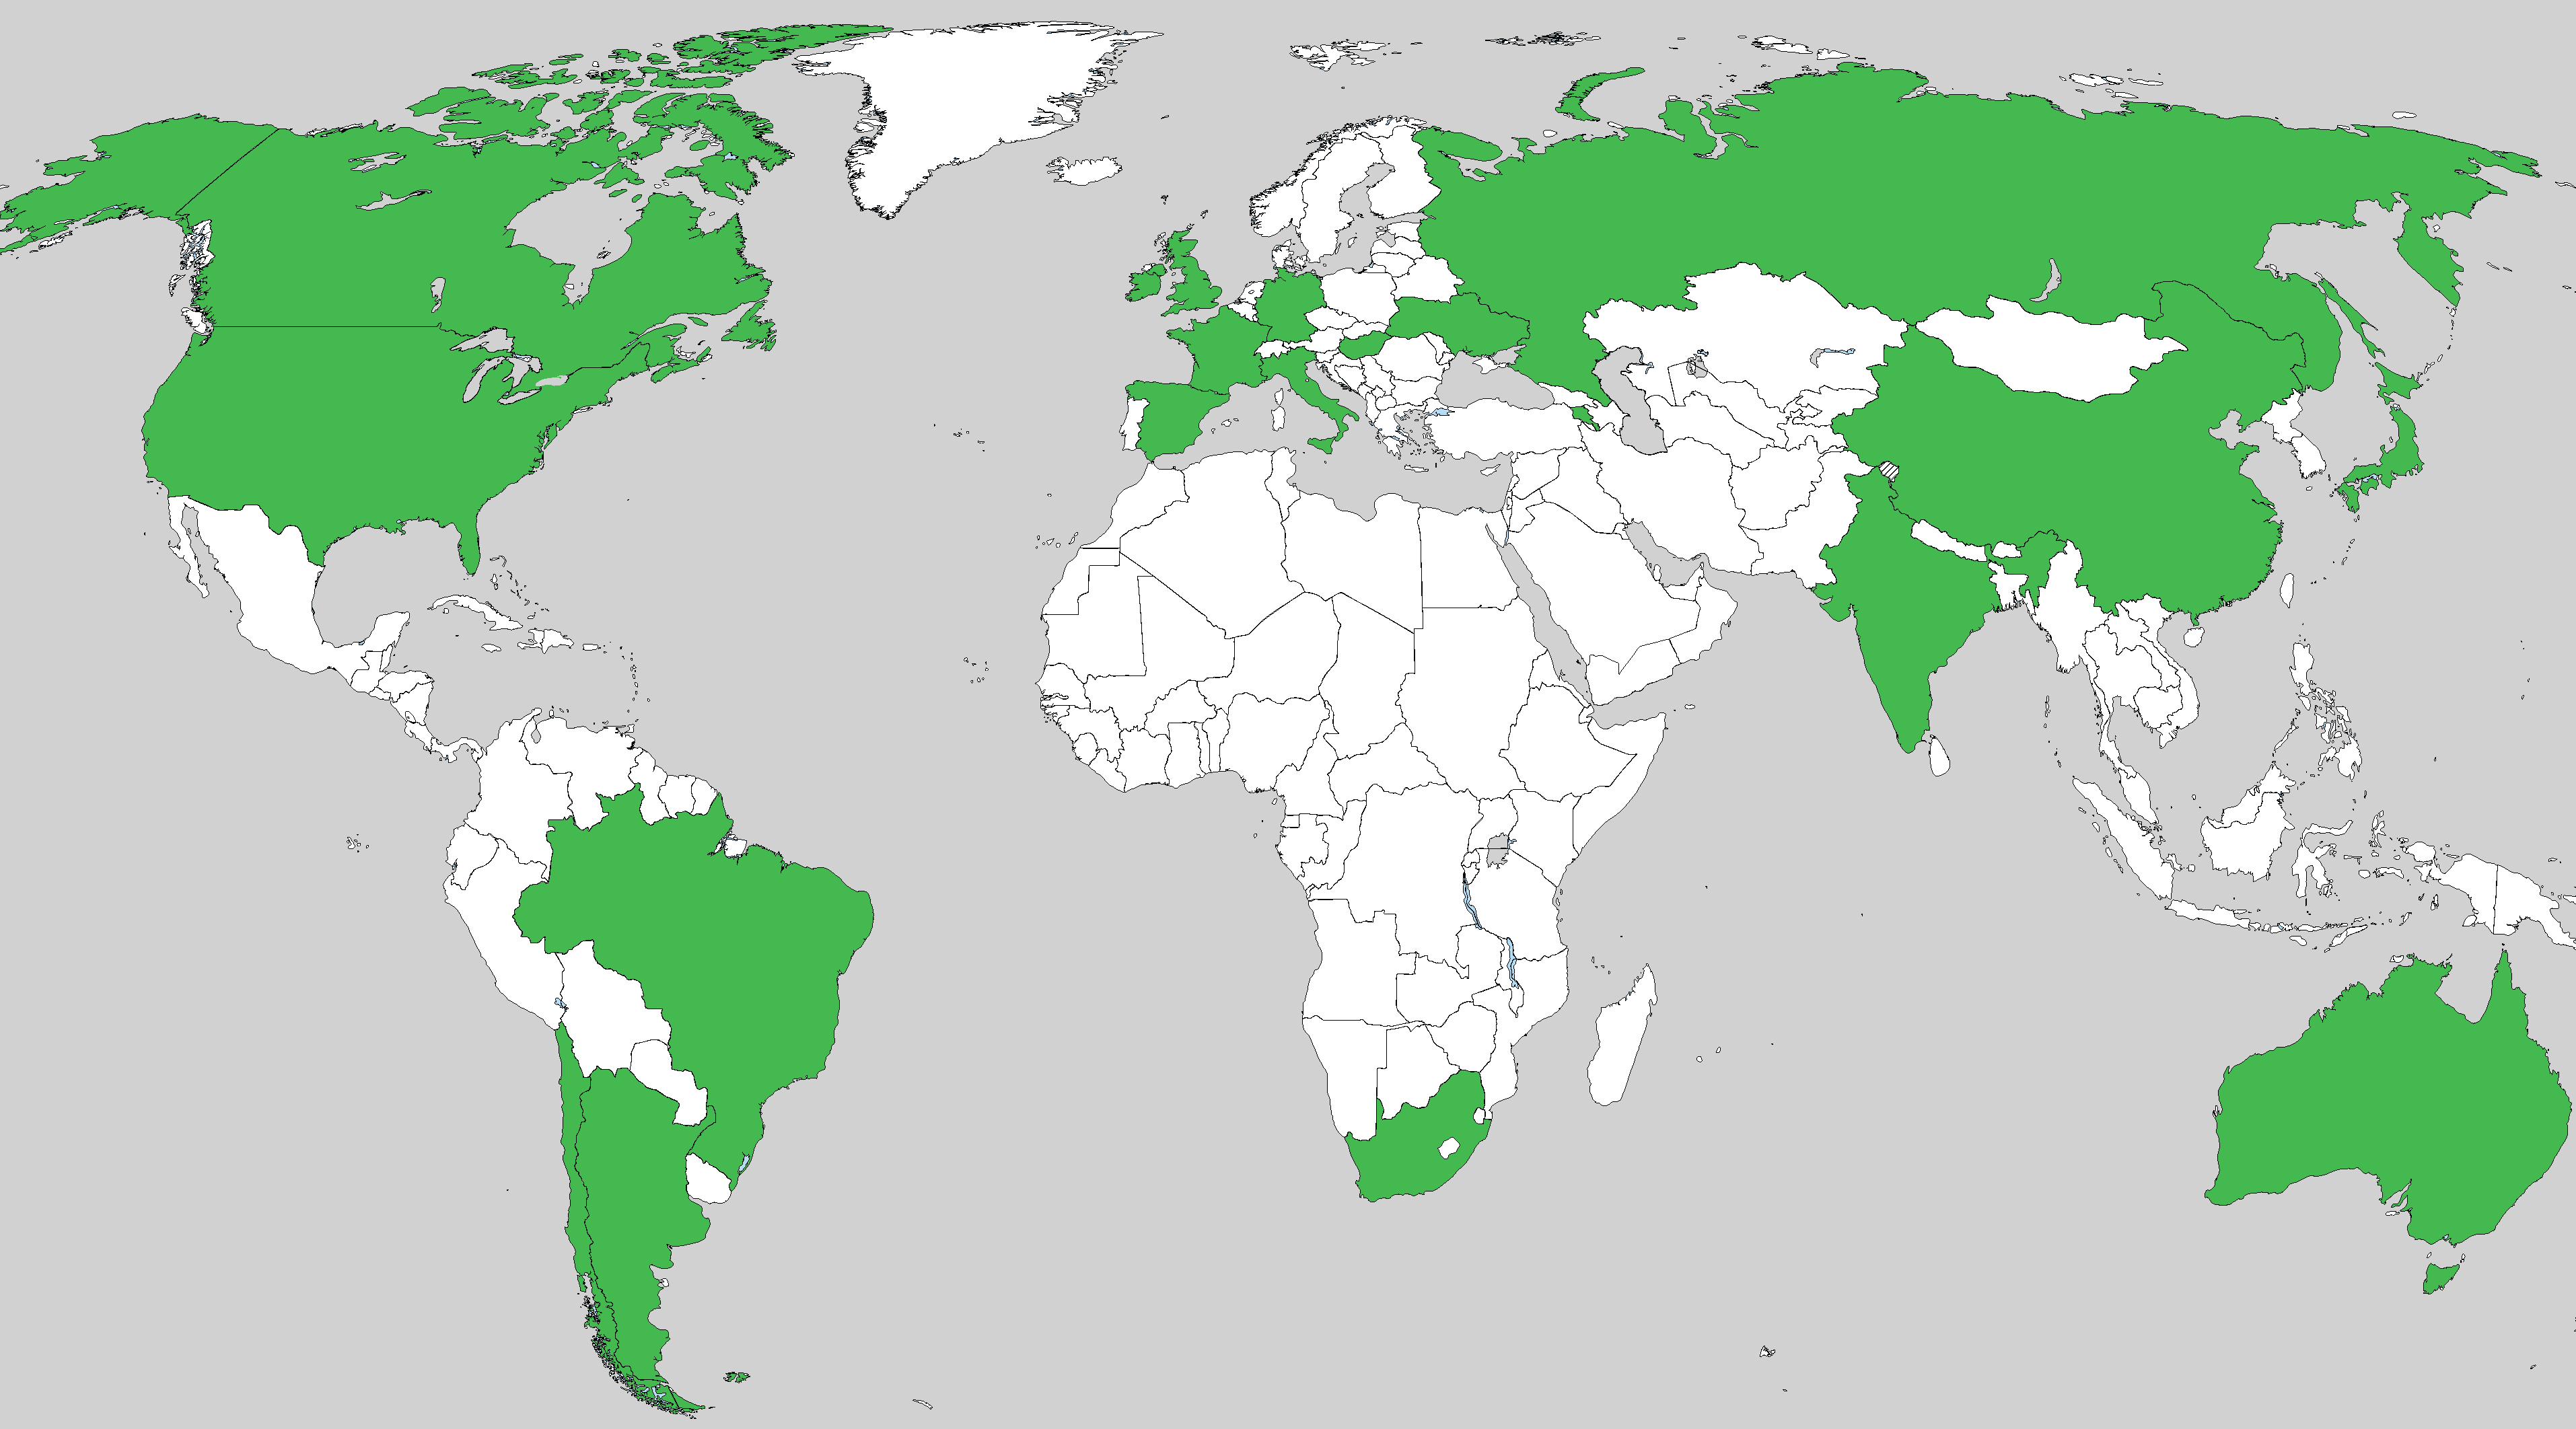
\includegraphics[width=0.9\linewidth]{img/VO-worldwide.png}
	\caption{International Virtual Observatory Alliance presence in the world.}
\label{figure:worldview}
\end{center}
\end{figure}

\subsection{The IVOA}

Since June 2002, different virtual observatory projects have come to integrate the
International Virtual Observatory Alliance (IVOA) under the \textbf{Guidelines
for Participation\footnote{\url{http://www.ivoa.net/documents/latest/IVOAParticipation.html}}}. 
These projects are funded through national and international programs, both governmental and 
private, in collaboration with various centers of scientific studies, universities and
others institutions. The members of the Virtual Observatory share
knowledge between them and the community in a standardized manner. They
themselves are who develop these standards for data exchange and
interoperability.

Table \ref{table:partners} shows the partners of IVOA up to
February 2014 that represents a nation, and in Figure~\ref{figure:worldview} the
presence of IVOA worldwide is shown. Also, two international organizations
are part of the VO, including the European Space Agency VO
(ESA-VO\footnote{http://www.sciops.esa.int/index.php?project=SAT\&page=ESAVOIntro})
and the EURO-VO~\footnote{http://www.euro-vo.org/}, which is a federation of several VOs in Europe.
The founders and first members are the same countries that have
been developing astronomy and astronomical instruments in the world, 
such as in Eastern Europe, North America, east Asia and Oceania. During the last few years,
new VOs in other regions were integrated to IVOA, specially in the southern
hemisphere, like the two youngest members: South Africa and Chile. 
This offers not only a better worldwide coverage, but the chance of
better exploiting the high-quality data produced by observatories 
located in those countries, both locally and globally. 

\subsection{IVOA Architecture}

A Virtual Observatory (VO) is a framework that helps to solve several
problems faced by the world wide astronomical community.
One of this problems is related to have access to generated data by
different instruments. Therefore, an architecture
\footnote{\texttt{http://www.ivoa.net/documents/Notes/IVOAArchitecture/}} was designed by the IVOA, which is composed by
standards and protocols, that allow the transparent
and unified access to astronomical data servers. The IVOA Architecture
defines 3 layers:
\begin{itemize}
        \item the \textbf{Resource Layer} consists in a server
collection with data from different instruments,
        \item the \textbf{User Layer} where astronomers and researchers can
search for data through different mechanisms,
        \item and the \textbf{Middle Layer} which allows the connection
between the previous two layer, hiding all the complexity for the
users. Thus, they can find data through the \emph{Registry}, or get the data
through \emph{Data Access} protocols.
\end{itemize}

\begin{figure}%[h]
\begin{center}
	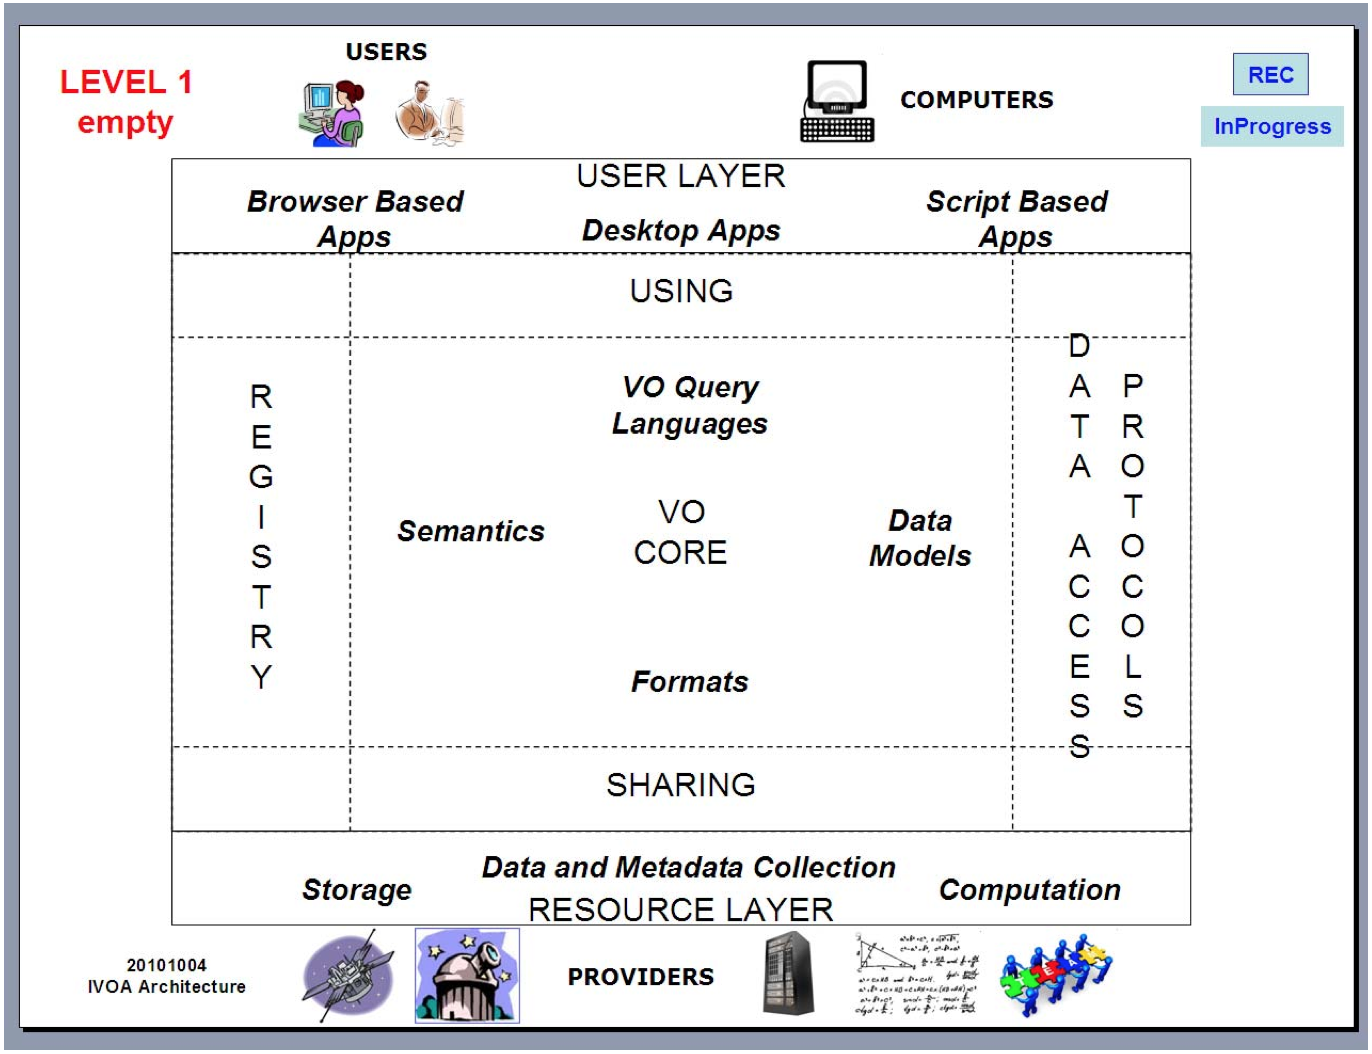
\includegraphics[width=0.9\linewidth]{img/ivoa_arch.png}
	\caption{IVOA Architecture.}
\end{center}
\label{figure:ivoarch}
\end{figure}

\subsection{Working groups}

For the creation and update of standards and protocols, IVOA is organized
by working groups. The description of each standard can be
found in IVOA website\footnote{http://www.ivoa.net/members/}. 
Currently, IVOA is organized in the following \textbf{Working Groups}:
\begin{itemize}
\item \textbf{Applications}:it is concerned primarily with the software
	tools that astronomers use to access VO data an services.
\item \textbf{Data Access Layer}: define and formulate VO standards for
	remote access, oriented to publishers and clients functionalities.
\item \textbf{Data Modeling}: provide a framework for the description
	of metadata attached to observed or simulated data.
\item \textbf{Grid and Webservices}: define the use of grid technologies
	and web services within the VO context.
\item \textbf{Resource Registry}: allow an astronomer to be
	able to locate, get details, and use, any resource located 
	anywhere in the VO.
\item \textbf{Semantics}: explore the word  and sentences
	meaning or interpretation, or another language forms in the
	astronomical context.
\item \textbf{VO Event}: define the content and meaning of a
	standard information packet for representing, transmitting, 
	publishing and archiving information about a transient celestial event.
\item \textbf{VOTable}: maintenance of an XML format, defined
	for the exchange of tabular data in the context of the VO.
\end{itemize}


\subsection{Popular Standard and Services}
\label{sec:popservices}

The working groups described above, have defined several standards
and recommendations that each VO node should implement. A standard usually 
define a basic set of elements to be implemented in order
to be IVOA compliant, but it also define recommendations of optional
elements and protocols. A clear distinction can be made between those
standards that define service protocols, and those that define data models
language descriptions or other internal implementation details.

Currently, the most popular \emph{services} are those defined for
the \textbf{Data Access Layer} (right side of Figure~\ref{figure:ivoarch}), 
probably because recovering data is the first thing that a VO node must offer.
We highlight here the four most used ones:
\begin{itemize}
\item \textbf{SCS}: Simple Cone Search, a query that describes a sky position and a
angular distance, defining a cone on the sky where to search for resources.
\item \textbf{SIA}: Simple Image Access, a query that defines a rectangular region on
the sky where to find images.
\item \textbf{SSA}: Simple Spectral Access, an interfaces to remotely discover
and access one-dimensional spectra. 
\item \textbf{TAP}: Table Access Protocol, a service protocol for accessing
general table data. The access is provided for both database and table metadata
as well as for actual table data.
\end{itemize}

On the other hand, identifying the most used ``non-service'' standards is much
more subjective, because specific implementations are much complex to verify
than services, and no all the VO nodes accurately report their IVOA compliance. 
Regardless this, we highlight here four ``non-service'' standard that are usually important
to consider:
\begin{itemize}
\item \textbf{ADQL}: Astronomical Data Query Language, a query language strongly
based on SQL92 that include astronomy specific operations. 
\item \textbf{ObsCoreDM}: Observation Core Data Model, a data structure
containing the basic information used by standard query services such as SCS.
\item \textbf{VOTable}: Virtual Observatory Table, a XML standard for the
interchange of astronomical data represented as a set of tables, loosely based 
in the FITS table standard.
\item \textbf{VOSpace}: Virtual Observatory Space, the IVOA interface to
distributed storage that host persistent and interchangeable data.
\end{itemize}


%The founder members of IVOA a In the southern hemisphere, 

%Almost half of IVOA virtual observatories are supported in Europe:
%\footnote{The
%Observatoire Virtuel France is ommited in \textbf{Europe} subsection of
%\textbf{List of Virtual Observatories} section by lack of the information.} 
%9 of
%the total; 1 belong to Africa, 1 to Australia, 2 to North America, 3 to South
%America and 5 to Asia. 


%\begin{figure}%[h]
%\begin{center}
%	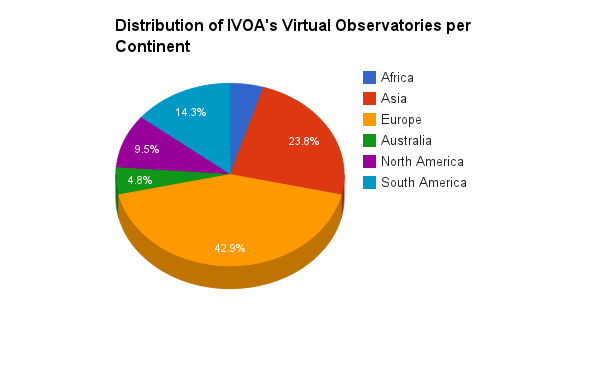
\includegraphics[scale=0.6]{img/vo_distribution.png}
%	\caption{International Virtual Observatory Alliance distribution per
%             continent.}
%\end{center}
%\end{figure}

%<<<<<<< HEAD

%=======
%\begin{figure}%[h]
%\begin{center}
%	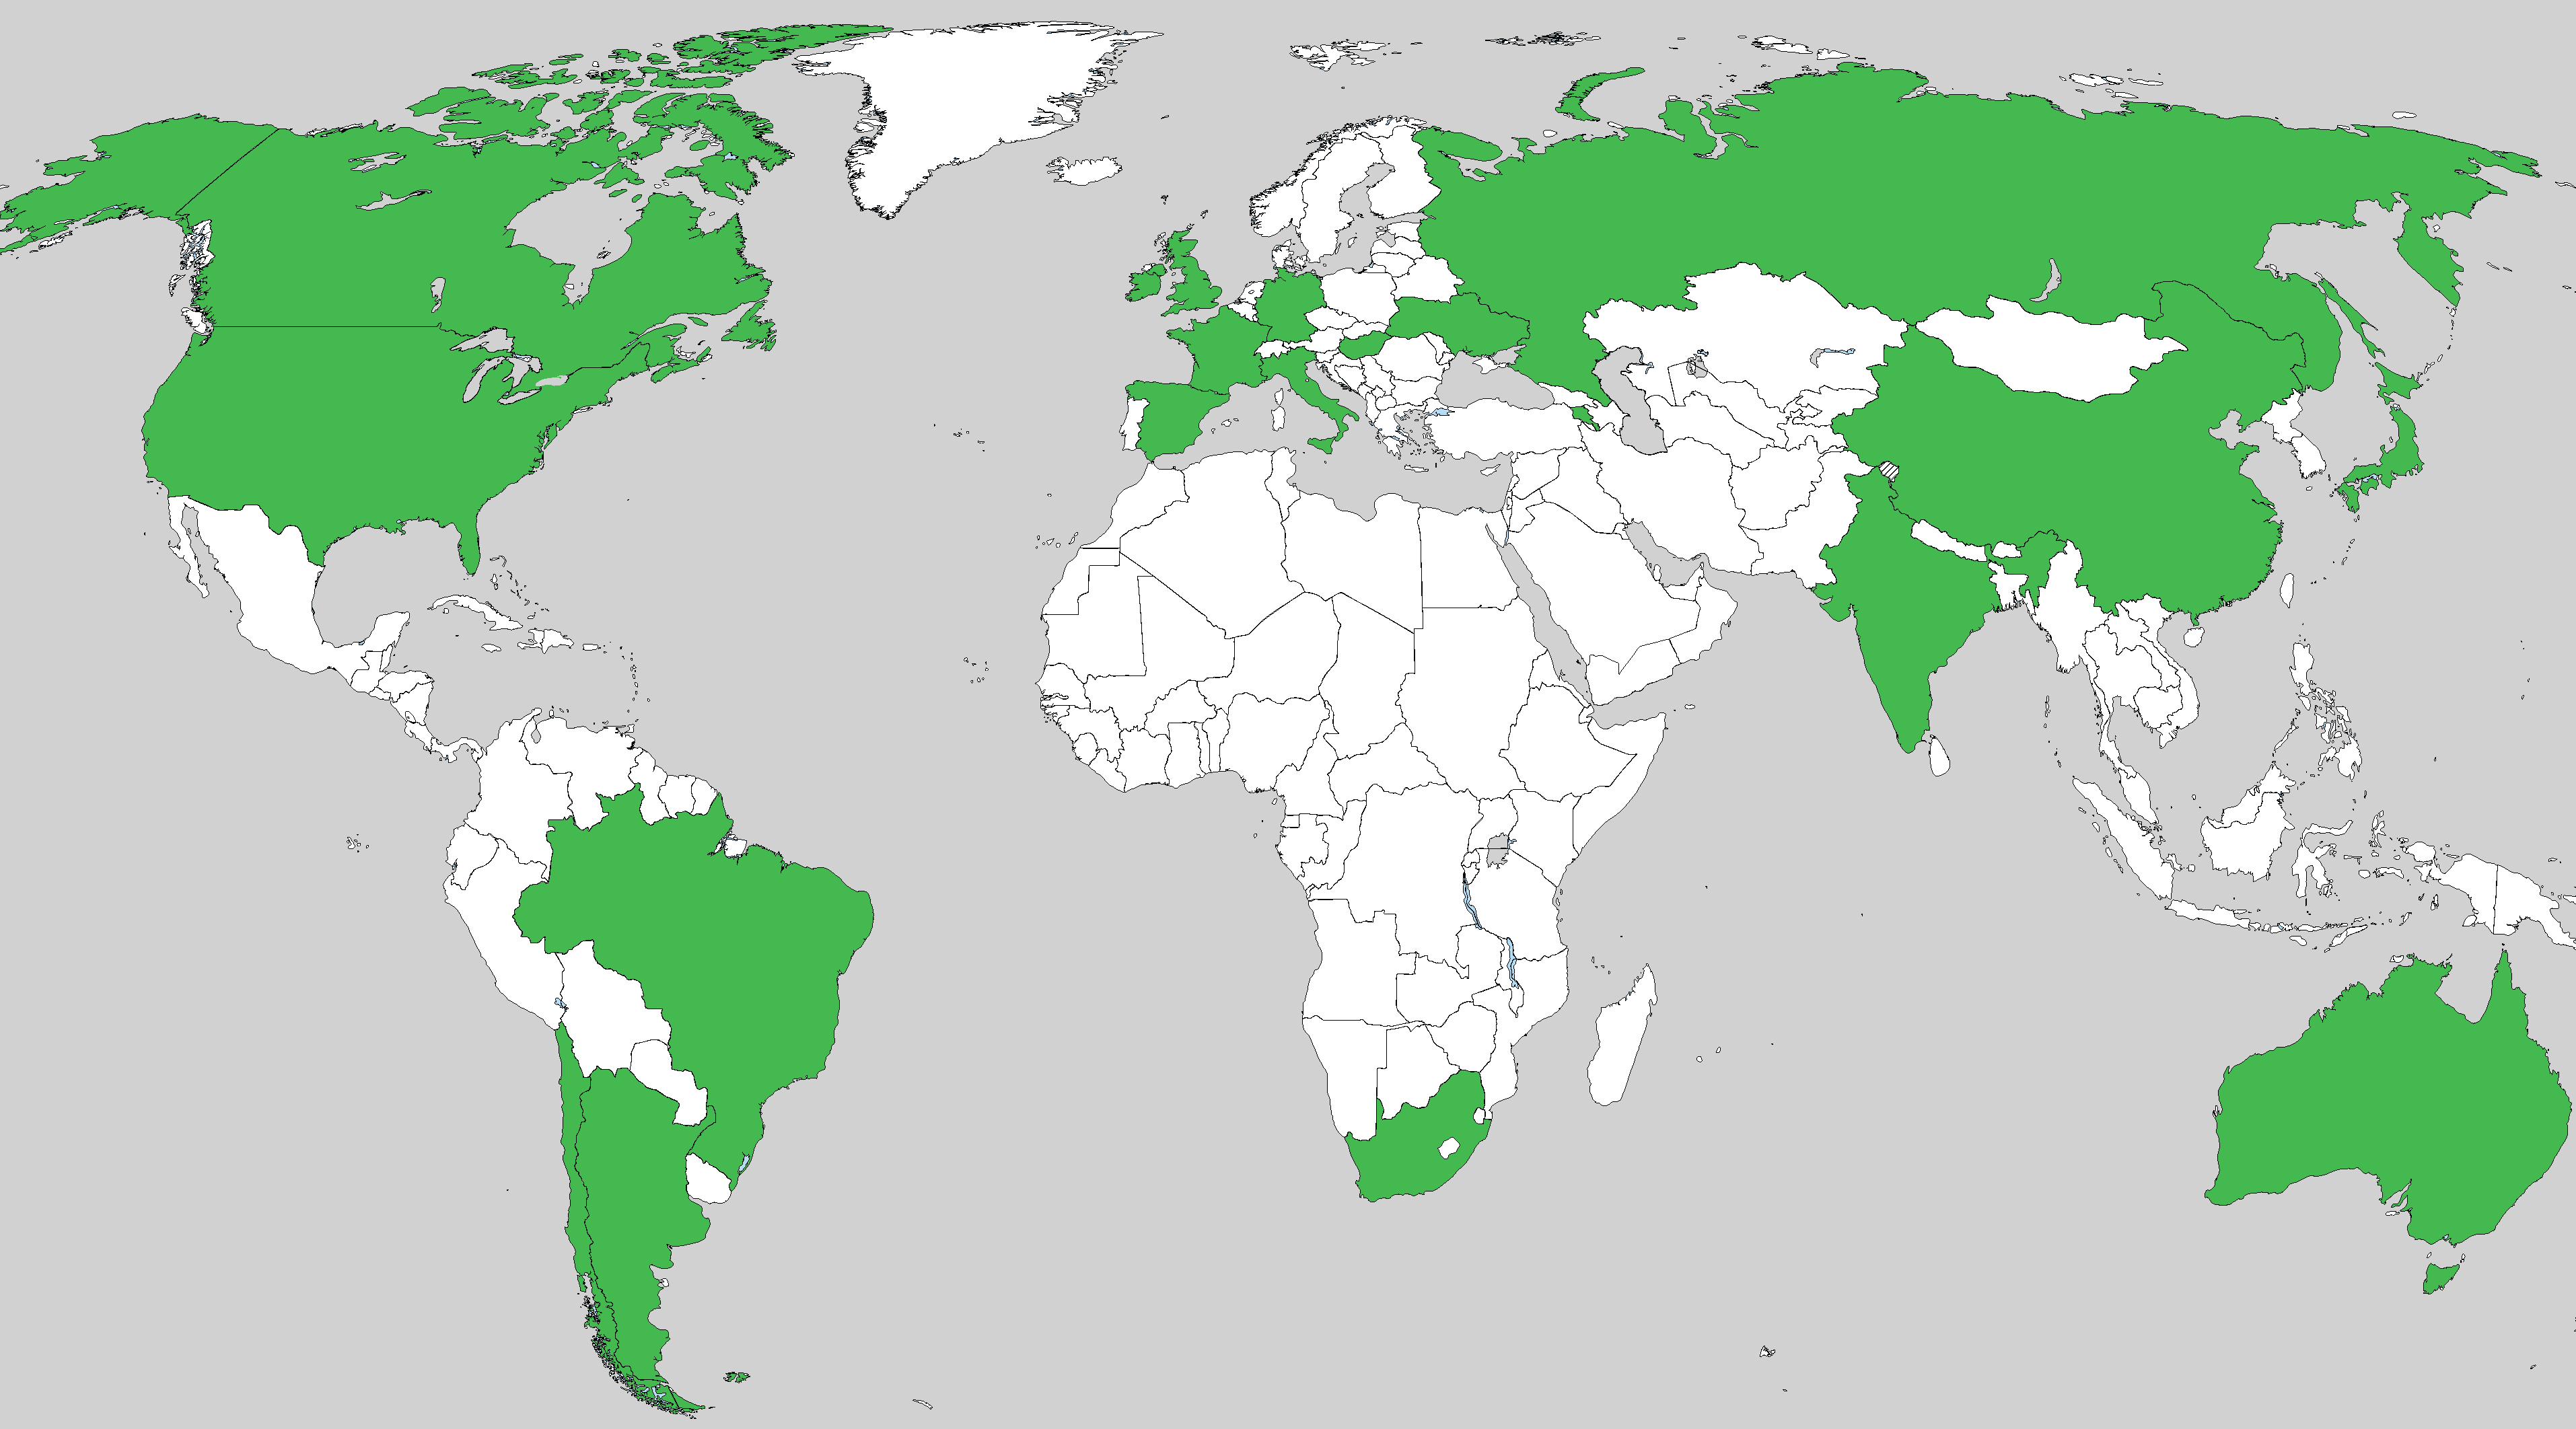
\includegraphics[width=0.9\linewidth]{img/VO-worldwide.png}
%	\caption{International Virtual Observatory Alliance presence in the world.}
%\end{center}
%\end{figure}
%
%\rem{JA}{A lot of initiatives converges in one and only VO. Access worldwide to 
%scientists.}

%\rem{MA}{subsec: Put here the infrastructure and the organizations}
%>>>>>>> 3def46e3eefecbe775b056101750c01287231178
%\subsection{Infrastructure}
%\begin{itemize}
%\item \textbf{EURO-VO}
%\item \textbf{EURO-VO Data Centre Alliance (EuroVO-DCA)}:
%it is supported by the European Union (EU) in the framework of the FP6
%e-Insfraestructure Communication Network Development initiative (project
%RI031675). It began on 1st of September, 2006, and ended on 31th of December,
%2008.
%\item \textbf{EURO-VO Astronomical Infraestructure for Data Access
%              (EuroVO-AIDA)}:
%it is supported by the European Union (UE) in the framework of the FP7
%e-Infrastructure Scientific Research Repositories initiative (%project
%RI2121104). It began on 1st of February, 2008, and ended on 31th of July, 2010.
%\end{itemize}

%<<<<<<< HEAD
%=======
%\subsection{Organizations}
%\rem{MA}{Funding and Support: important actors of a VO}
%\begin{itemize}
%	\item \textbf{CVO}
%	\item Canadian Astronomy Data Centre
%	\item \textbf{VAO}
%	\item National Science Foundation, NSF
%	\item National Aeronautics and Space Administration, NASA 
%	\item Associated Universities, Inc, AUI.
%	\item Association of Universities for Reseach in Astronomy, AURA
%	\item \textbf{BRAVO}
%	\item Brazilian Astronomical Society, SBA
%	\item National Institue for Science and Technology in Astrophysics, INCT-A
%	\item \textbf{ChiVO}
%	\item 5 universities, supported by ALMA, REUNA
%	\item \textbf{NOVA}
%	\item 8 institutions, National Universitiy of La Plata, Faculty of Astronomical 
%		Sciences and Geophysics of la Plata
%	\item \textbf{ArVO}
%	\item Digital First Byurakan Survey, DFBS
%	\item \textbf{AstroGrid}
%	\item Particle Physics and Astronomy and Research Council  (PPARC)
%	\item Sciency \& Technology Facilities Council (STFC)
%	\item \textbf{ESA-VO}
%	\item Study
%	\item \textbf{EURO-VO}
%	\item Continuation of Astrophysical Virtual Observatory, European Commision and six organization
%	\item \textbf{GAVO}
%	\item Federal Ministry of Education and Research (BMBF)
%	\item \textbf{SVO}
%	\item Centro de Astrobiología (INTA-CSIC)
%	\item Artificial Intelligence Department of the National University of Distance Education
%	\item University of Cádiz and Center of Scientific and Academic Services of Catalonia (CESCA)
%	\item \textbf{VObs.it}
%	\item Italian National Institute for Astrophysics
%	\item Information System Units
%	\item \textbf{Ukrainian}
%	\item Ukrainian Astronomical Association (UAA)
%	\item \textbf{SA$^3$}
%	\item National Research Fundation
%	\item South African Astronomical Observatory
%	\item Hartebeesthoek Radio Astronomy Observatory
%	\item Square Kilometer Array South Africa 
%	\item \textbf{China-VO}
%	\item National Astronomical Observatories
%	\item Chinese Academy of Sciences
%	\item \textbf{JVO}
%	\item National Astronomical Observatory of Japan
%	\item Fujitsu
%	\item \textbf{VOI}
%	\item Inter University Center for Astronomy and Astrophysics
%	\item Ministry of Communication and Information Technology
%	\item \textbf{Aus-VO}
%	\item Linkage Infrastructure, Equipment and Facilities
%\end{itemize}
%>>>>>>> 3def46e3eefecbe775b056101750c01287231178



%\rem{MA}{subsec: Development lines of VOs and data speciality}

% If Chile became part of International Virtual Observatory Alliance, the
% distribution of IVOA's members per continent will be as shown in the figure
% 2. \\

%\begin{comment}
%\begin{figure}%[h]
%\begin{center}
%	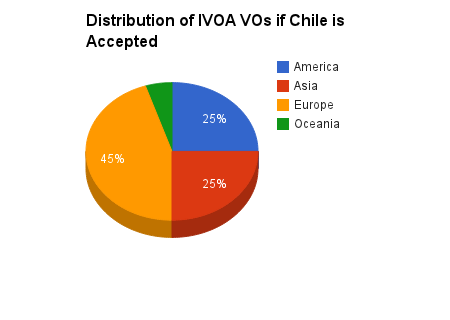
\includegraphics[width=110mm]{img/if_chile.png}
%	\caption{International Virtual Observatory Alliance distribution per
%             continent if Chile is accepted.}
%\end{center}
%\end{figure}
%\end{comment}

%Without considering the status of the internal projects of the virtual
%observatories, the membership of Chile would contribute to the cooperation,
%development and interoperability from America in the same percent that Asia.
%Furthermore, this fact would be very significant, because a large numbers of
%astronomical centers like observatories are placed in this country.  For now, is
%intended to work with a certain quantity of data of ALMA.\\


